%#!pdfplatex
\documentclass{article}
\usepackage{graphicx}
\title{Fundamental Exercise on Computer and Information Engineering 1B \\ Image Processing}
\author{XL15613   Thiago Machado da Silva}
\date{\today}

\begin{document}
\maketitle

\section*{Source codes}
\subsection*{Header files}
Refer to Figure~\ref{fig:headers}. \\
Each {\tt .c} file that don't have a {\tt main} function has an {\tt .h} header file with the same name. They usually have {\tt ifdef}, {\tt define} and {\tt endif} to make sure each header is accounted only once. Also external functions have their prototypes in header files. \\
\begin{figure}[h]
  \makebox[\textwidth][c]{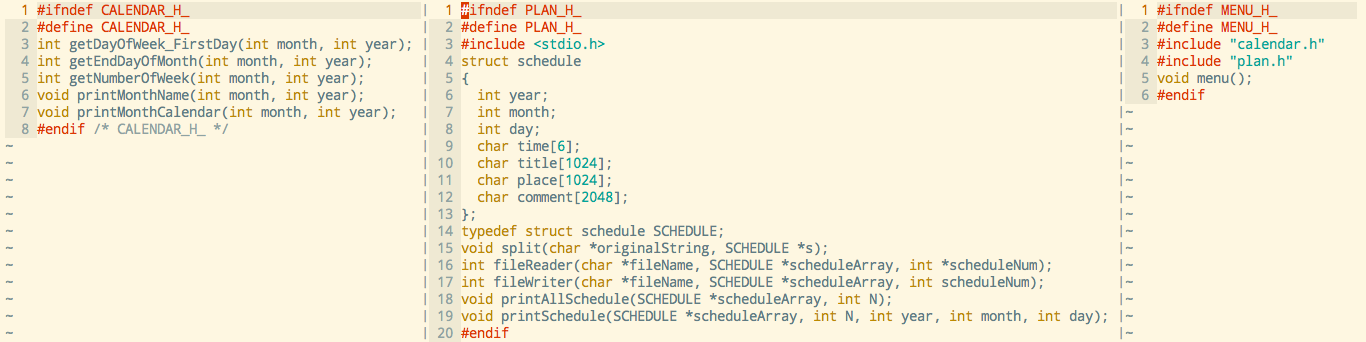
\includegraphics[width=1.78\textwidth]{./img/headers.png}}%
  \centering
  \caption{from left to right: {\tt calendar.h}, {\tt plan.h} and {\tt menu.h}.}
  \label{fig:headers}
\end{figure}

\subsection*{Calendar}
Refer to Figure~\ref{fig:calendar}. \\
Some constant variables were created, mostly for similar data usage. \\
There is one bad practice where a {\tt bool} value is used as an {\tt int} value, in {\tt getEndDayIfMonth} function, resulting in a small size function. \\
There is an extra printing in {\tt printMonthCalendar} function, where the week day name is also printed. \\
\begin{figure}[h]
  \makebox[\textwidth][c]{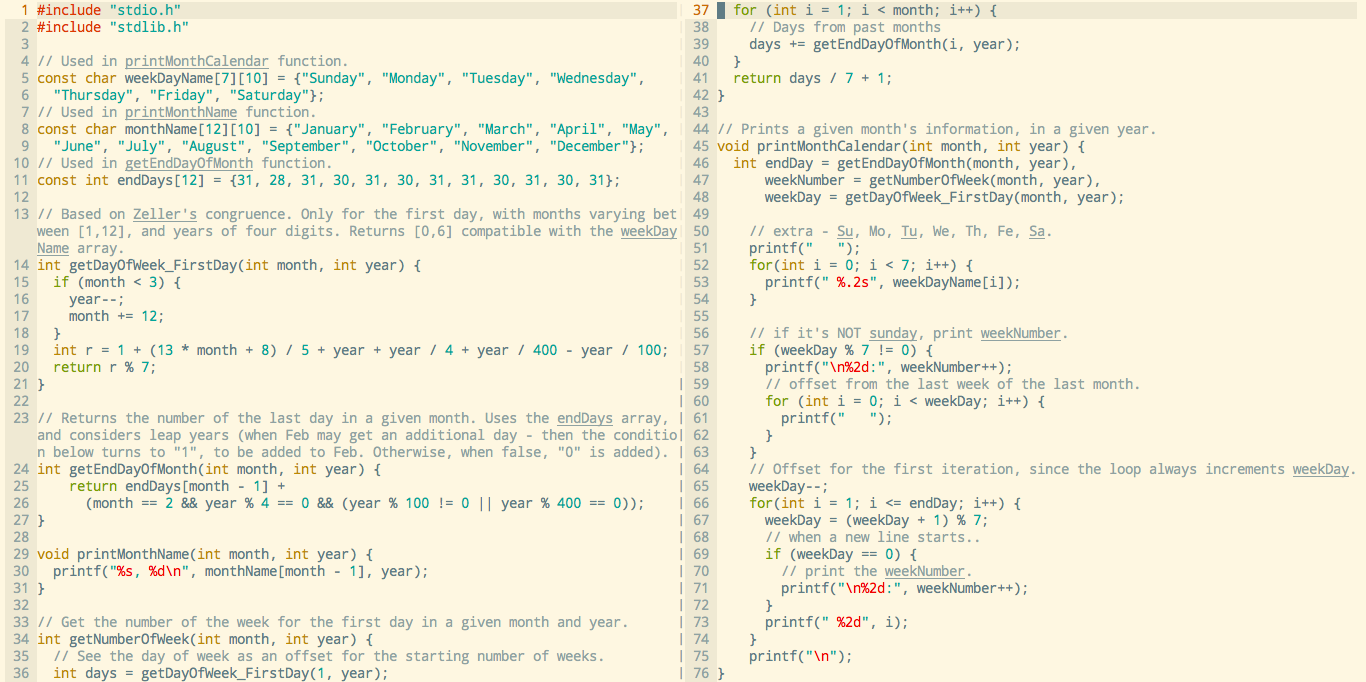
\includegraphics[width=1.78\textwidth]{./img/calendar.png}}%
  \centering
  \caption{{\tt calendar.c}.}
  \label{fig:calendar}
\end{figure}

\subsection*{Plan}
Refer to Figure~\ref{fig:plan}. \\
In this file, there aren't a lot of data copying since pointers are heavily used, regarding the function's parameters initialization. \\
In {\tt split} function, the comment input is intended to be optional. If no commentary is detected, the {\tt comment} char vector is formated to be an "empty string". \\
\begin{figure}[h]
  \makebox[\textwidth][c]{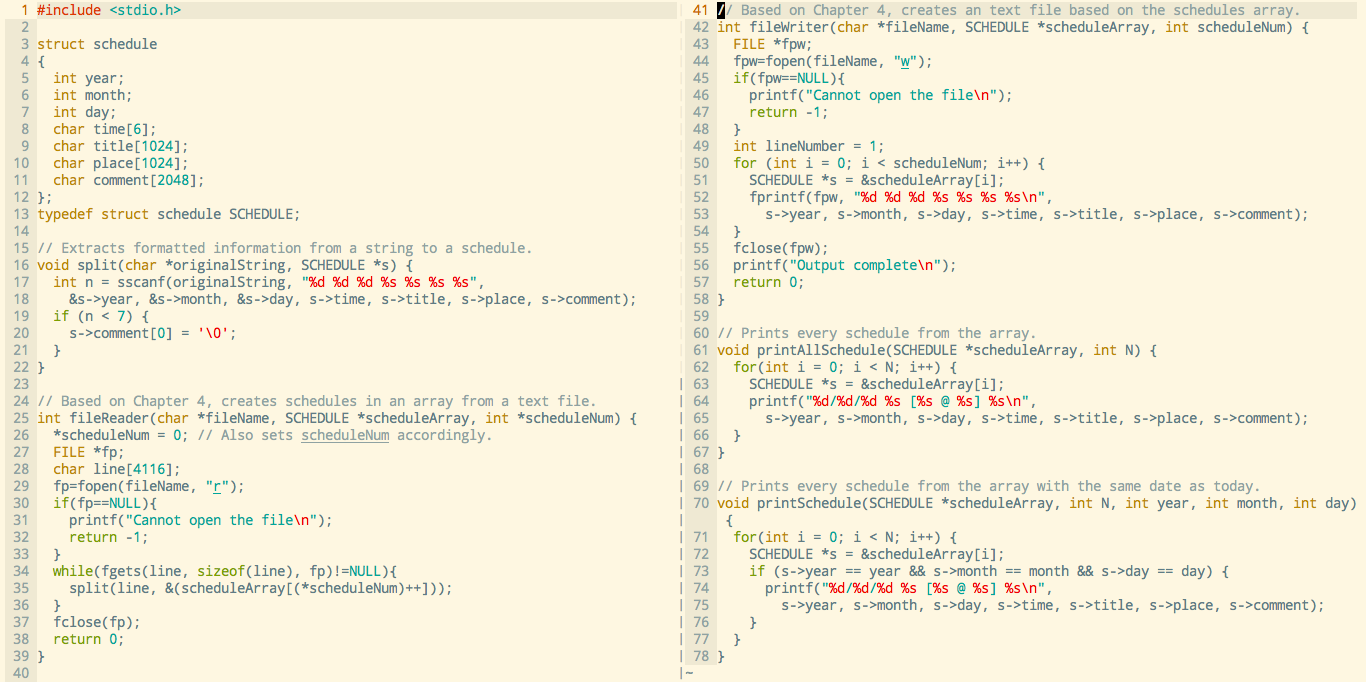
\includegraphics[width=1.78\textwidth]{./img/plan.png}}%
  \centering
  \caption{{\tt plan.c}.}
  \label{fig:plan}
\end{figure}

\subsection*{Menu}
Refer to Figure~\ref{fig:menu}. \\
Some constant data are declared in the top of the code. \\
A {\tt valid} function is implemented. It returns {\tt 1} for valid and {\tt 0} for invalid, even though I think it's a good practice to use {\tt true} for valid and {\tt false} for invalid. \\
In {\tt menu} function, There'd be less memory de/allocation if I declared {\tt s} ({\tt SCHEDULE*} type) outside of the {\tt for} loop. But this variable lifetime is enclosed in a small scope, where it is actually used, and I consider this an advantage. \\
\begin{figure}[h]
  \makebox[\textwidth][c]{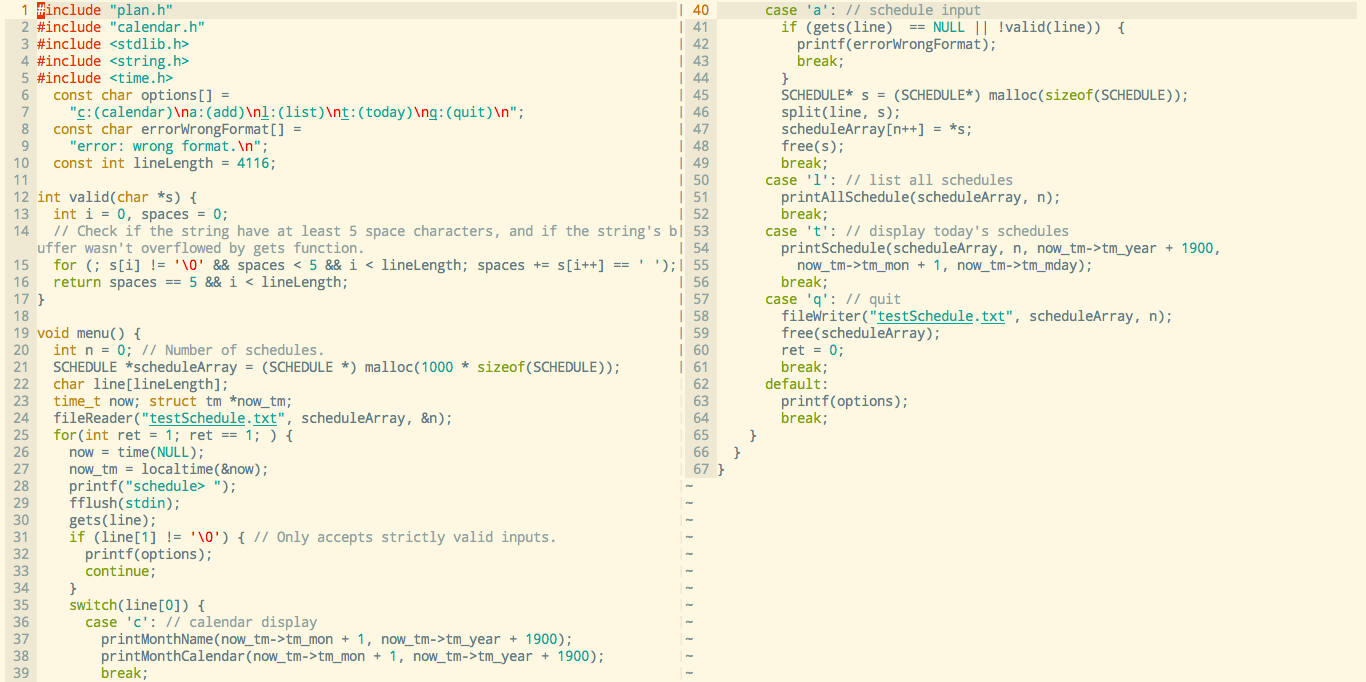
\includegraphics[width=1.78\textwidth]{./img/menu.png}}%
  \centering
  \caption{{\tt menu.c}.}
  \label{fig:menu}
\end{figure}

\section*{calImpl3}
Refer to Figure~\ref{fig:calImpl3}. \\
The commands show, from the left pane to the right pane: Compilation, testing the existence of {\tt testSchedule.txt}, then {\tt calImpl3} execution. Then in the right pane, another {\tt testSchedule.txt} existence test, then two more {\tt calImpl3} executions.
\begin{figure}[h]
  \makebox[\textwidth][c]{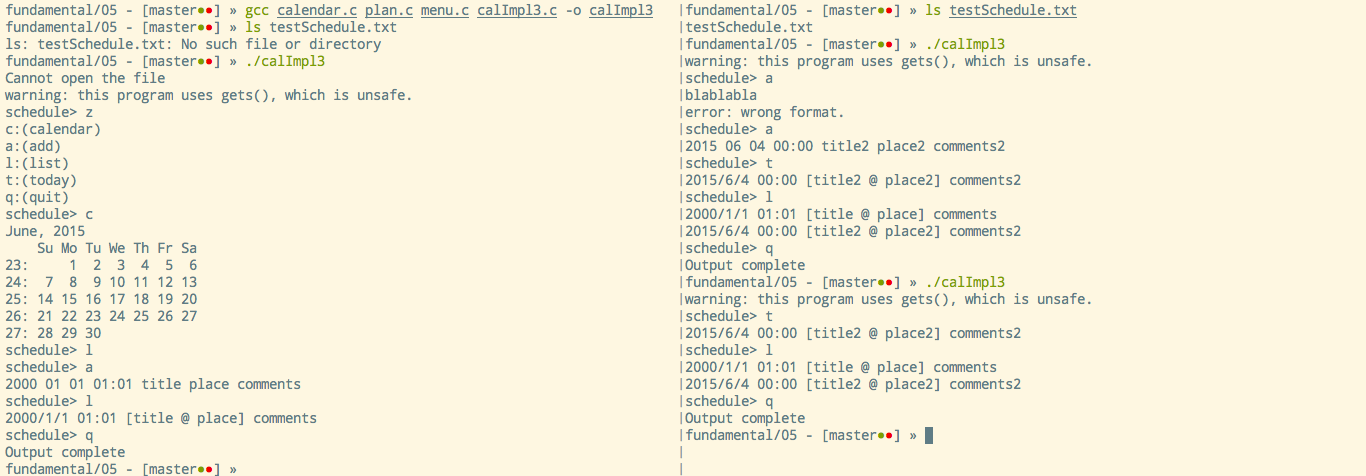
\includegraphics[width=1.78\textwidth]{./img/calImpl3.png}}%
  \centering
  \caption{Commands related to {\tt calImpl3} (compilation and some tests). First, the left pane were executed, then the right pane.}
  \label{fig:calImpl3}
\end{figure}
\end{document}
